\parag Primeiro é feita a análise dos componentes usando o multímetro e medidor de impedância do Elvis. Os resultados são dispostos na Tabela 1.

\vspace{5pt}
\begin{table}[h]
\centering
\begin{tabular}{|c|c|c|c|}
\hline
\textbf{Grandeza} & \textbf{Valor nominal} & \textbf{Valor medido} & \textbf{Erro (\%) }\\\hline
R & 47$\Omega$ & 47.359$\Omega$ & 0.76 \\\hline 
L & 1mH & 0.863mH & 13.70 \\\hline 
C & 100nF & 107.500nF & 7.50 \\\hline 
\end{tabular}
\caption*{Tabela 1: Valores dos componentes}
\end{table}

Em seguida, esses componentes são usados para montar o circuito exposto na Figura 1.

\begin{table}[h]
\centering
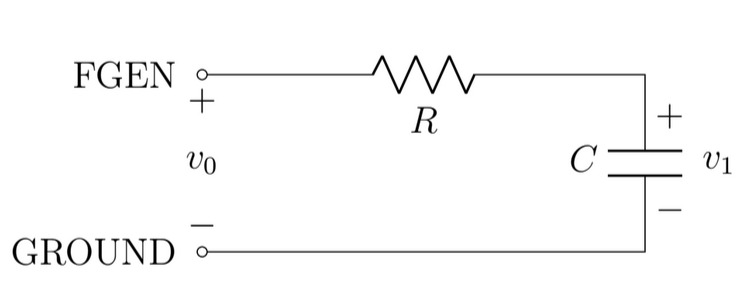
\includegraphics[scale=0.4]{figuras/figura1}
\end{table}
\begin{center}
Figura 1: Disposição do Circuito 1
\end{center}

O gerador de funções do Elvis é configurado para gerar uma onda triangular com 2$V_{pp}$, offset zero e frequência de 1kHz. Assim, é gerada a onda do Gráfico 1.

\begin{table}[h]
\centering
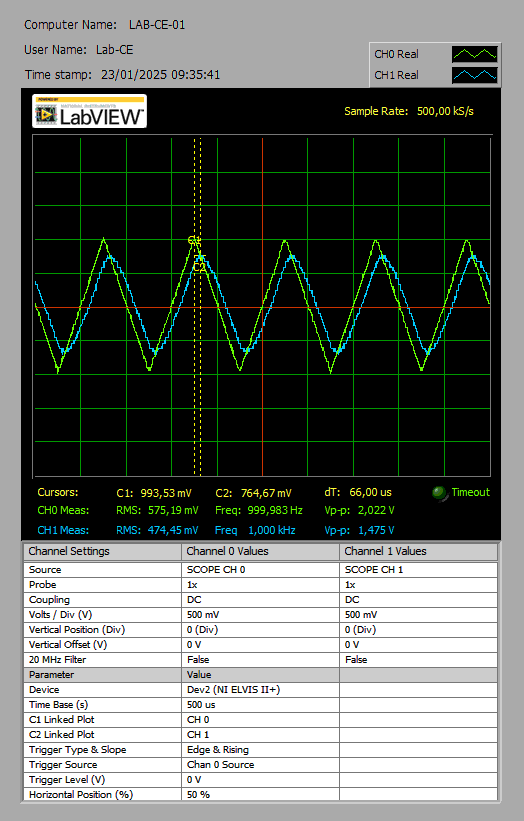
\includegraphics[scale=0.8]{graficos/rgadicoa1-triangulo}
\end{table}
\begin{center}
Gráfico 1: Onda Triangular
\end{center}

%calculo da serie de fourier da triangular

Em seguida, vamos calcular a resposta do sistema para os harmônicos de frequências 1, 3, 5, 7, 9, 11, 13, 15, 17 e 19 kHz.

%calculo

Agora experimentalmente são medidas as mesmas respostas, que seguem nos Gráficos 2 a 11. 

\newpage\begin{table}[h]
\centering
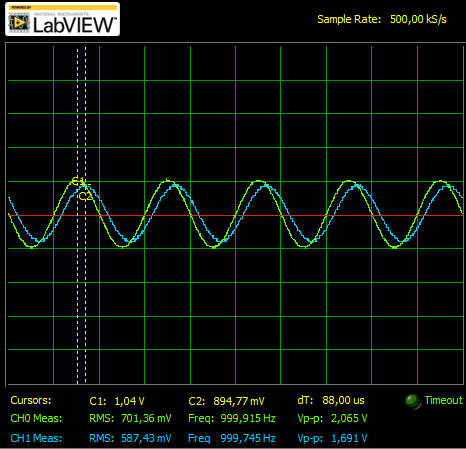
\includegraphics[scale=0.7]{graficos/RGADICOA1}
\end{table}
\begin{center}
Gráfico 2: Resposta para Frequência 1kHz
\end{center}


\begin{table}[h]
\centering
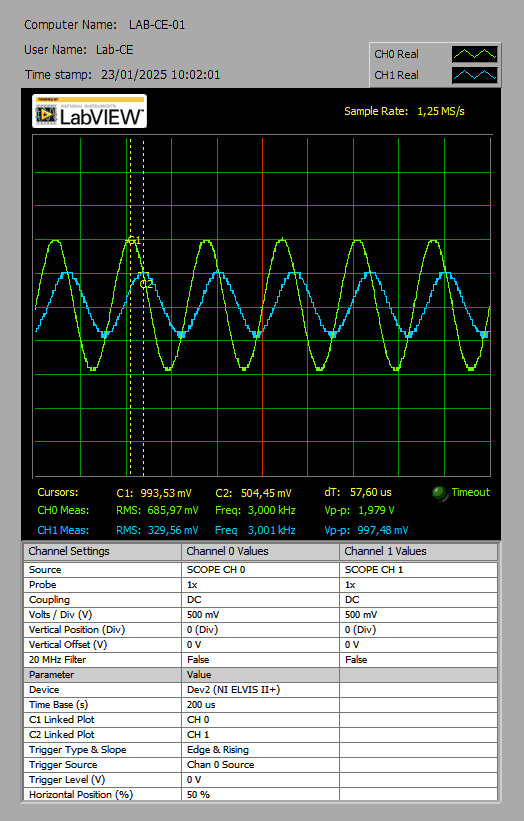
\includegraphics[scale=0.7]{graficos/RGADICOA3}
\end{table}
\begin{center}
Gráfico 3: Resposta para Frequência 3kHz
\end{center}

\newpage
\begin{table}[h]
\centering
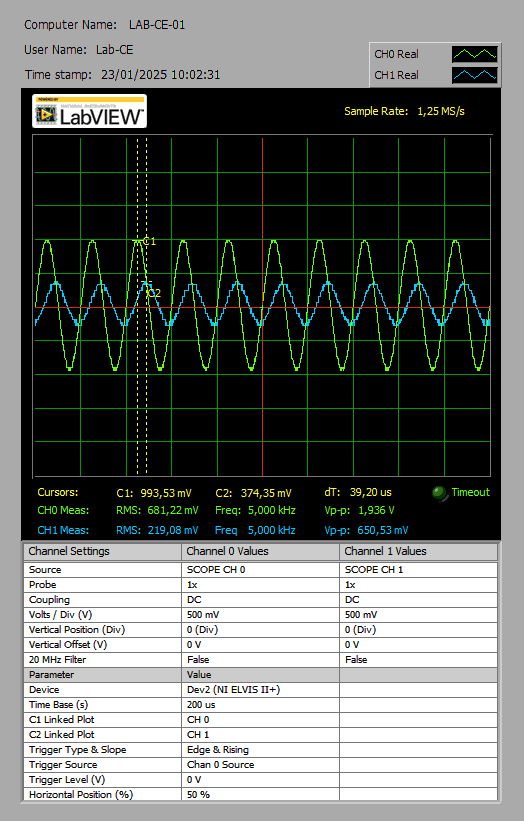
\includegraphics[scale=0.7]{graficos/RGADICOA5}
\end{table}
\begin{center}
Gráfico 4: Resposta para Frequência 5kHz
\end{center}


\begin{table}[h]
\centering
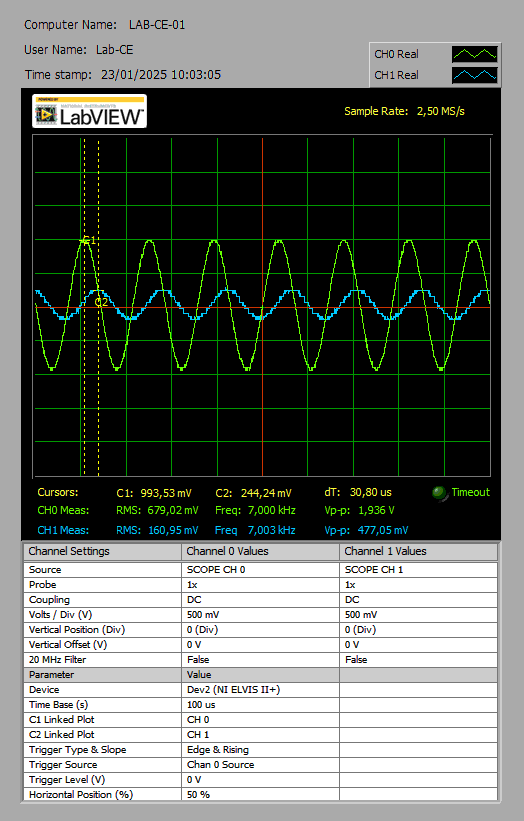
\includegraphics[scale=0.7]{graficos/RGADICOA7}
\end{table}
\begin{center}
Gráfico 5: Resposta para Frequência 7kHz
\end{center}

\newpage
\begin{table}[h]
\centering
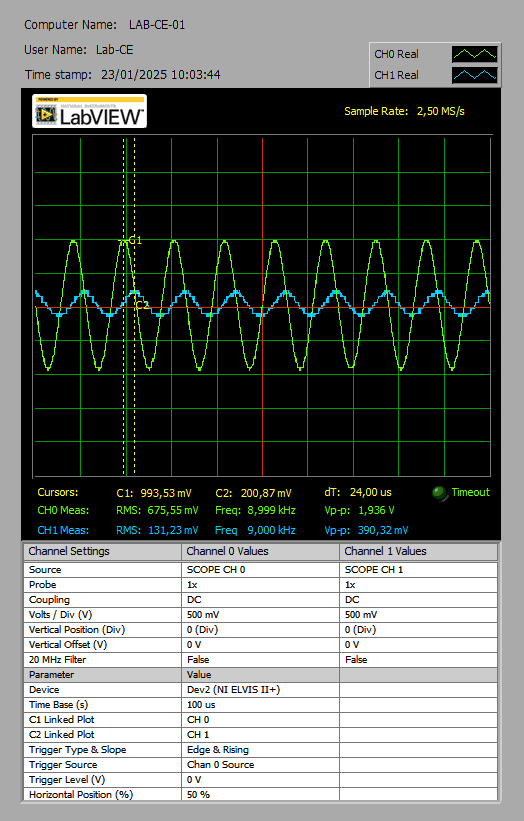
\includegraphics[scale=0.7]{graficos/RGADICOA9}
\end{table}
\begin{center}
Gráfico 6: Resposta para Frequência 9kHz
\end{center}


\begin{table}[h]
\centering
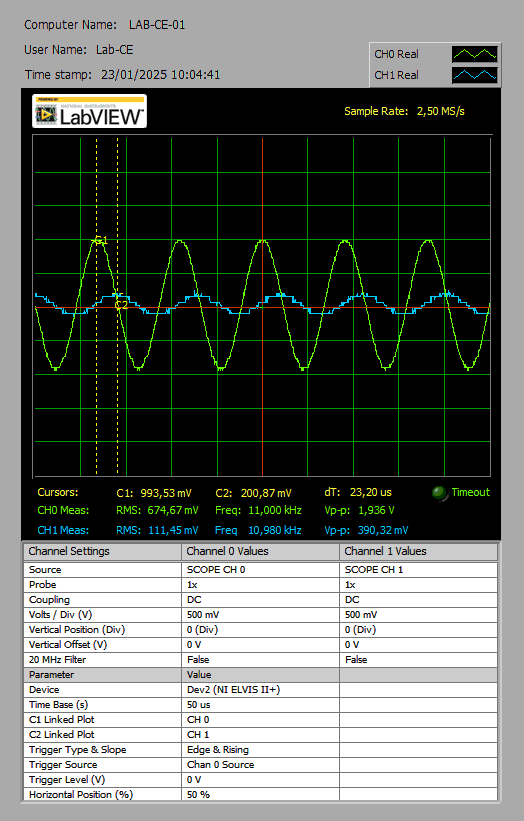
\includegraphics[scale=0.7]{graficos/RGADICOA11}
\end{table}
\begin{center}
Gráfico 7: Resposta para Frequência 11kHz
\end{center}

\newpage
\begin{table}[h]
\centering
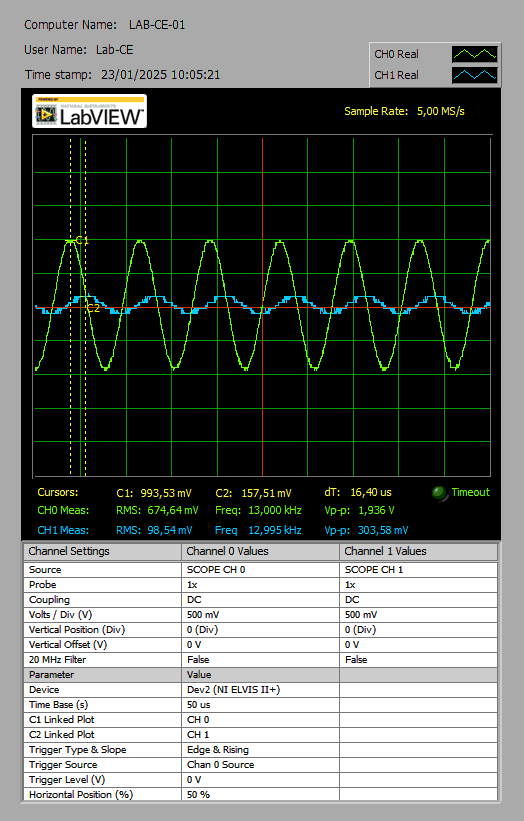
\includegraphics[scale=0.7]{graficos/RGADICOA13}
\end{table}
\begin{center}
Gráfico 8: Resposta para Frequência 13kHz
\end{center}


\begin{table}[h]
\centering
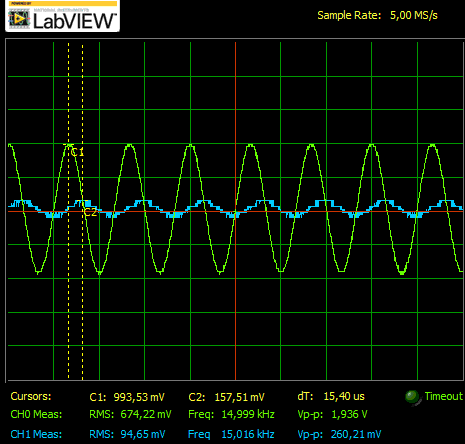
\includegraphics[scale=0.7]{graficos/RGADICOA15}
\end{table}
\begin{center}
Gráfico 9: Resposta para Frequência 15kHz
\end{center}

\newpage
\begin{table}[h]
\centering
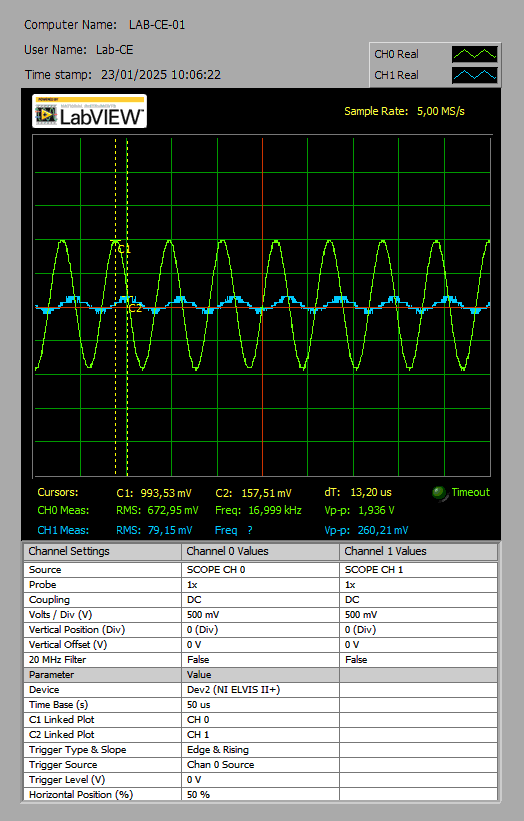
\includegraphics[scale=0.7]{graficos/RGADICOA17}
\end{table}
\begin{center}
Gráfico 10: Resposta para Frequência 17kHz
\end{center}


\begin{table}[h]
\centering
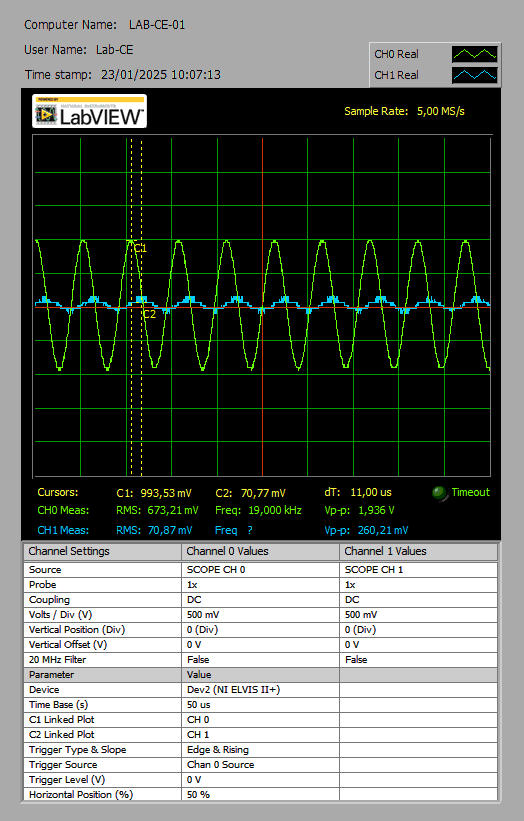
\includegraphics[scale=0.7]{graficos/RGADICOA19}
\end{table}
\begin{center}
Gráfico 11: Resposta para Frequência 19kHz
\end{center}